\pdfminorversion=5
\pdfobjcompresslevel=2

\RequirePackage[l2tabu, orthodox]{nag}

\documentclass[sigplan, screen]{acmart}

\usepackage[T1]{fontenc}
\usepackage[utf8]{inputenc}

\usepackage{microtype}
\usepackage{listings}
\usepackage{color}
\usepackage{xspace}
\usepackage{balance}
\usepackage{todonotes}
\usepackage{subcaption}
\usepackage[all]{nowidow}
\usepackage{tikz}
\usepackage[scaled]{beramono}
\usepackage{booktabs}
%\usepackage[bookmarks=false,colorlinks=true,allcolors=black,breaklinks]{hyperref}
\usepackage{cleveref} % Keep me last so that I can
                      % reset other counters

%\setlength{\belowcaptionskip}{-15pt} % Bear with me

\newtheorem{definition}{Definition}

% Copyright
%\setcopyright{none}
\setcopyright{acmcopyright}
%\setcopyright{acmlicensed}
%\setcopyright{rightsretained}
%\setcopyright{usgov}
%\setcopyright{usgovmixed}
%\setcopyright{cagov}
%\setcopyright{cagovmixed}

% DOI
%\acmDOI{10.475/123_4}

% ISBN
%\acmISBN{123-4567-24-567/08/06}

%Conference
\acmConference[SLE'18]{International Conference on Software Language Engineering}{November 2018}{Boston, MA, USA}
\acmYear{2018}
\copyrightyear{2018}

\acmPrice{15.00}

%\acmBadgeL[http://ctuning.org/ae/ppopp2016.html]{ae-logo}
%\acmBadgeR[http://ctuning.org/ae/ppopp2016.html]{ae-logo}

\hypersetup{%
	pdftitle={},
	pdfauthor={},
	pdfkeywords={}
}

% Usual suspects
\newcommand*{\ie}{i.e.,\@\xspace}
\newcommand*{\eg}{e.g.,\@\xspace}
\newcommand*{\cf}{cf.\@\xspace}

\makeatletter
\newcommand*{\etc}{%
	\@ifnextchar{.}%
	{etc}%
	{etc.\@\xspace}%
}
\makeatother

\newcommand*{\de}{$\Delta$\@\xspace}
\newcommand*{\ds}{$\Delta$s\@\xspace}
\newcommand*{\db}{$\Delta$-based\@\xspace}
\newcommand*{\M}{\mathcal{M}}

\newcommand*{\diff}{\textit{diff}\@\xspace}
\newcommand*{\patch}{\textit{patch}\@\xspace}
\newcommand*{\prism}{\textsc{Prism}\@\xspace}

% Listings
\definecolor{keywordscolor}{RGB}{127, 0, 85}
\definecolor{stringcolors}{RGB}{42, 0, 255}
\definecolor{commentscolor}{RGB}{63, 127, 95}
\definecolor{annotationscolor}{RGB}{100, 100, 100}
\definecolor{lstbgcolor}{RGB}{245, 245, 245}

% Custom Java
\lstset{
	language=Java,
	%	mathescape=true,
	literate={->}{$\rightarrow$}{1},
	keywordstyle=\color{keywordscolor}\bfseries,
	commentstyle=\color{commentscolor},
	stringstyle=\color{stringcolors},
	basicstyle=\ttfamily\tiny,
	captionpos=b,
	numbers=left,
	%	backgroundcolor=\color{lstbgcolor},
	%	framexleftmargin=20pt,
	xleftmargin=17pt,
	aboveskip=\bigskipamount,
	belowskip=\bigskipamount,
	%	frame=tb,
	tabsize=2,
	breaklines=true
}

% Rascal
\lstdefinelanguage[]{Rascal}[]{Java}
{
	morecomment=[l]{\@},
	morekeywords={alias, tuple, lrel, data, str, value, int, list}
}

\usetikzlibrary{shapes.callouts, shadows}
\tikzset{author comment/.style={draw, fill=white, thick, drop shadow}}

\newcommand{\Comment}[3]{%
	\ifthenelse{\boolean{CommentON}}{%
		\raisebox{-.5ex}
		{\tikz
			\node[x=1ex, y=1ex, inner sep=.5ex,
			rectangle callout,
			callout pointer width=.7ex,
			callout relative pointer={(1.5,-0)},
			author comment]
			{\footnotesize\textsf{#1}};}~%
		\textsf{[}\,\textcolor{#2}{#3}\,\textsf{]}\xspace
	}{} %else
}

\newcommand{\td}[1]{\Comment{TD}{blue}{#1}}
\newcommand{\fc}[1]{\Comment{FC}{red}{#1}}


\newboolean{CommentON}
\setboolean{CommentON}{true} % to disable the comments set CommentON to false in the main doc

\begin{document}
\title{Shape-Diverse DSLs:~Languages without Borders}
%\titlenote{Just brainstorming}
%\title{Towards Shape-diverse languages}
%\titlenote{Models are synchonized, not DSLs, though}
%\subtitle{Language Engineering across Technological Boundaries}
%\subtitlenote{Language Engineering without Borders}
%\subtitlenote{The full version of the author's guide is available as
%		\texttt{acmart.pdf} document}

\author{Fabien Coulon}
\affiliation{
	\institution{University of Toulouse, IRIT \& Obeo}
	\city{Toulouse}
	\country{France}
}
\email{fabien.coulon@obeo.fr}

\author{Thomas Degueule}
\affiliation{
	\institution{CWI}
	\city{Amsterdam}
	\country{Netherlands}
}
\email{degueule@cwi.nl}

\author{Tijs van der Storm}
\affiliation{
	\institution{CWI \& University of Groningen}
	\city{Amsterdam}
	\country{Netherlands}
}
\email{storm@cwi.nl}

\author{Benoit Combemale}
\affiliation{
	\institution{Univ. Toulouse, IRIT \& Inria}
	\city{Toulouse}
	\country{France}
}
\email{benoit.combemale@irit.fr}

% The default list of authors is too long for headers.
%\renewcommand{\shortauthors}{B. Trovato et al.}

\begin{abstract}
%
Domain-Specific Languages (DSLs) manifest themselves in remarkably diverse \emph{shapes}:~from internal DSL embedded as a mere fluent API within a programming language to external DSLs with dedicated syntax and tool support engineered using one of many language workbenches.

%
Theoretically, this diversity should enable language designers to combine the strengths of multiple language engineering technologies in the development of a single DSL, and enable language users to manipulate their abstractions in the most appropriate shape for the task at hand (\eg~domain modeling vs. system integration).

%
In practice, however, combining multiple language implementation techniques is problematic.
Language designers usually commit to a particular technology (\eg~Spoofax, EMF, Racket) and a particular shape (\eg~internal, external, API) early in the language design process and this choice can hardly be reconsidered later on.

%
In this vision paper, we report on early experiments and lessons learned building an incremental synchronization mechanism for \emph{metamorphic DSLs}.
Metamorphic DSLs are languages whose different constituents (syntax, semantics, tools) can be defined independently using various language engineering technologies and which can adapt their shape to a particular user or task.
Taking as example a simple metamorphic FSM language implemented simultaneously in three technological spaces (Rascal, EMF, a fluent API in Java), we show how the same FSM models can be manipulated indifferently under various shapes (a textual program in Rascal, a graphical projection in EMF, a Java AST).
This opens up the possibility to, \eg animate an FSM model in EMF while it is executed by an interpreter written in Rascal.

%
%Our approach relies on a communication bus that ships changes on a model (\emph{patches}) from one shape to the others.
%This opens up the possibility to, \eg, animate an FSM model in EMF while it is executed by an interpreter written in Rascal.
%Our approach caters for specificities of said technological spaces by allowing every shape to maintain extra shape-specific state (\eg~layout information in textual and graphical editors, runtime state).

%
We intend to raise the awareness of the community on the notion of metamorphic DSL, identify some of the challenges we encountered along the way and, hopefully, encourage future investigations.
\end{abstract}


%
% The code below should be generated by the tool at
% http://dl.acm.org/ccs.cfm
% Please copy and paste the code instead of the example below.
%
\begin{CCSXML}
	<ccs2012>
	<concept>
	<concept_id>10011007.10011006.10011050.10011017</concept_id>
	<concept_desc>Software and its engineering~Domain specific languages</concept_desc>
	<concept_significance>500</concept_significance>
	</concept>
	</ccs2012>
\end{CCSXML}

\ccsdesc[500]{Software and its engineering~Domain specific languages}

%\keywords{domain-specific language, metamorphic dsl, language workbenches}

%\begin{teaserfigure}
%	\includegraphics[width=\textwidth]{sampleteaser}
%	\caption{This is a teaser}
%	\label{fig:teaser}
%\end{teaserfigure}

\maketitle

\section{Introduction \& Motivating Example}
\td{Since we do not mention metamorphic DSLs in title/abstract anymore, mention them here}
One of the first steps in designing a new Domain-Specific Language (DSL) is to choose which \emph{language vehicle} (LV) will be used to engineer it.
We define a LV as the technological means for implementing a language.
This include language workbenches as well as programming languages and ontology languages, to name but a few.
%A language vehicle may pertain to any \emph{technological space} (TS) such as grammarware, modelware, PLware, \etc.
The notion of language vehicles is orthogonal to the distinction between \emph{technological spaces} (\eg~grammarware, modelware, PLware~\cite{kurtev2002technological}); between graphical and textual syntax; between internal, embedded, and external DSLs,~\etc.
%\footnote{In this paper, we build upon \citeauthor{kurtev2002technological}'s view of a TS:~``a working context with a set of associated concepts, body of knowledge, tools, required skills, and possibilities''~\cite{kurtev2002technological}.}
%In addition, we consider a cohesive set of tools in a given TS (\eg~a particular language workbench) as a separate TS.
For instance, following this definition, we consider Rascal~\cite{klint2010easy} and Spoofax~\cite{kats2010spoofax} as two distinct language vehicles within the broader technological space of grammarware and meta-programming; EMF~\cite{steinberg2008emf} and UML~\cite{fowler2004uml} as two distinct language vehicles within the broader technological space of modelware.
LVs usually come with their own meta-languages for expressing the various aspects of a DSL:~abstract syntax, concrete syntax, static and execution semantics, tools, \etc.
%Examples of prominent LV include meta-modeling environments such as EMF~\cite{steinberg2008emf}, meta-programming environments such as Rascal~\cite{klint2010easy} and Spoofax~\cite{kats2010spoofax}, projectional environments such as MPS~\cite{voelter2013language}, plain old programming languages such as Racket~\cite{felleisen2018programmable} or Scala~\cite{hofer2010modular}, and language workbenches (LWBs) in general~\cite{erdweg2015evaluating}.
%\td{Sentence above could be shortened/removed}
As implementation techniques radically differ from one LV to another, this initial design choice commits the development of a DSL in a set direction that can hardly be reconsidered later on.

From the language designer's point of view, however, every LV has its own strengths.
The ecosystem around EMF excels in the definition of, for instance, graphical editors and persistence frameworks for large models, while the Rascal environment excels in the definition of, for instance, interpreters and refactoring tools.
%On the other hand, the flexibility of manipulating the concepts of a DSL through a fluent API, using the capabilities of a general-purpose programming language, is unmatched.
The benefits of various LV are also visible from the language users' point of view.
While domain experts may prefer to manipulate domain concepts through a dedicated syntax, advanced users (\eg~system integrators) may favor the flexibility of a fluent API in their favorite programming language to manipulate the very same abstractions.
%However, it is currently not possible to \emph{combine the strengths of multiple LV to engineer a single DSL}.
%\td{Why?}

Let us consider a simple finite-state machine (FSM) language as a motivating example.
As depicted in \Cref{fig:motivating-fsm}, one would like to combine the strengths of multiple LVs to engineer this DSL.
Rascal could be used to develop its interpreter, a set of refactoring tools (\eg~state collapsing and minimization), and a textual editor; EMF to develop a graphical simulator for running FSM models; Java to offer a fluent API for advanced users who focus on its integration with other DSLs or within a broader system.

\begin{figure}[bt]
	\centering
	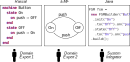
\includegraphics[width=\columnwidth]{figures/motivating-fsm-simplified}
	\caption{Three incarnations of the same FSM model in three language vehicles:~different representations and tools for different users and tasks.}
	\label{fig:motivating-fsm}
\end{figure}

Using today's techniques, it is possible to define the same FSM language in these three LV separately.
It is not possible, however, to apply the tools of a given LV on the models created in another LV---for instance, animating a FSM model written in EMF using the Rascal interpreter, or synchronizing a textual FSM model in Rascal with its equivalent incarnation in the form of a Java AST.
Achieving this goal requires to synchronize the diverse in-memory representations of the same model in different LV; for instance to let the Rascal interpreter update its in-memory representation of an FSM model and synchronize it with the in-memory representation of the same model in EMF.

In this paper, we envision a language engineering activity where language designers combine tools from multiple vehicles to engineer a single DSL.
We endeavor to show \emph{how to break down the barriers between different vehicles so that language designers can combine the strengths of each in the engineering of a single DSL, and language users can synchronize their models across various shapes}.
%\emph{Metamorphic synchronization} refers to the possibility of synchronizing different incarnations of the same model in different shapes of a language, \ie~in different vehicles.
%As different vehicles rely on radically different theories, a successful approach for bridging them must thus \emph{align} \td{!no!} them in some way.

We first present our approach, \prism, in \Cref{sec:prism}, and then highlight our implementation of the shape-diverse FSM language in \Cref{sec:eval}.
Finally, we discuss the research challenges we identify and next steps in \Cref{sec:discussion}.
       % Why
\section{Shape-diverse DSLs}
\label{sec:shapes}

The cornerstone artifact defining a DSL in any LV is its abstract syntax.
The way abstract syntax is expressed differs drastically from one LV to another: GEMOC~\cite{bousse2016execution} and Xtext~\cite{bettini2016implementing} use Ecore metamodels~\cite{steinberg2008emf}; MPS~\cite{voelter2014generic} uses \emph{concepts}; Rascal~\cite{klint2010easy} uses Algebraic Data Types (ADT); \etc.
Language embedding techniques, on the other hand, use the constructs of an host language to materialize the abstractions of a DSL in the host language itself (\eg~a set of Java classes).
Concrete models are then built as instances of the corresponding abstract syntax formalism:~Ecore models, ADT values, Java ASTs, \etc.
The tools defined within a particular LV (an interpreter in Rascal, an editor in EMF) manipulate models in the corresponding formalism (respectively, ADT values and Ecore models).
These formalisms radically differ in many ways:~object-oriented vs. functional, graphs vs. trees, mutable ASG vs. immutable ASTs, cross-references vs. symbolic names, \etc.
As LVs are developed by independent groups of people and rely on different underlying theories, it is neither possible nor desirable to establish a common formalism upon which all LVs would agree.

%\Cref{fig:concepts} gives an overview of the concepts we use throughout this paper.
%A ``conceptual'' language $\mathcal{L}$ is materialized as a shape $\mathcal{S}$ in a LV.
%$\mathcal{S}$ can therefore be seen as the implementation of $\mathcal{L}$ in the LV.
%Similarly, a ``conceptual'' model $m$ conforming to $\mathcal{L}$ is materialized as an incarnation $\mathcal{I}$ conforming to the shape $\mathcal{S}$ in a LV.
%\td{Not very proud of the ``conceptual''. Is ``abstract'' better? Any idea?}
%\fc{Language Specification and Abstract Model?}
%As each shape manipulate models in its own formalism, all incarnations $I$ of the same model $m$ must remain synchronized.
%
%A naive way to bridge different LVs would be to define bidirectional transformations between the abstract syntax formalisms of every pair $\langle LV, LV' \rangle$.
%Doing so however would close the world around the chosen set of LVs.
%As every LV holds particular extra information on its incarnations, such as layout in an editor, runtime data for running models, or context information around API calls, the synchronization must be incremental.
%
%In our approach, \prism, every change occuring on one incarnation is shipped to all other incarnations of the same model.
%Every shape \fc{LV responsibility?} is responsible for\dots

\begin{figure}[bt]
	\centering
	
\includegraphics[width=.6\columnwidth]{figures/shape-diverse-lang}
	\caption{Languages are implemented as shapes in LVs as well as Models are realized as incarnations in corresponding LVs. Just as models conform to languages, incarnations conform to shapes.}
	\label{fig:concepts}
\end{figure}

\Cref{fig:concepts} gives an overview of the concepts we use in this paper to address this problem.
A ``conceptual'' language $\mathcal{L}$ is materialized as a \emph{shape} $\mathcal{S}$ in a LV.
$\mathcal{S}$ can therefore be seen as the implementation of $\mathcal{L}$ in the LV.
As mentioned earlier, Ecore metamodels, ADT definitions, and Java APIs are examples of shapes.
Similarly, a ``conceptual'' model $m$ conforming to $\mathcal{L}$ is realized as an incarnation $\mathcal{I}$ conforming to the shape $\mathcal{S}$ in a LV: an Ecore model, an ADT value, or a Java AST.
%\td{Not very proud of the ``conceptual''. Is ``abstract'' better? Any idea?}
%\fc{Language Specification and Abstract Model?} 
Synchronization must thus happen between the various incarnations of a model, such as the ones depicted in \Cref{fig:motivating-fsm}.
%As each shape manipulate models in its own formalism, all incarnations $I$ of the same model $m$ must remain synchronized.

%An obvious way to bridge different LVs would be to define bidirectional transformations between the abstract syntax formalisms of every pair $\langle LV, LV' \rangle$.
%Doing so however would close the world around the chosen set of LVs.
%As every LV holds particular extra information on its incarnations, such as layout in an editor, runtime data for running models, or context information around API calls, the synchronization must be incremental.

This synchronization mechanism must ensure two important properties.
First, it must not close the world around a chosen set of LVs:~it should be possible to easily plug new LVs and shapes to meet new requirements from users and designers.
This rules out any synchronization approach that would require to be defined for every pair $\langle LV, LV' \rangle$, such as bidirectional transformations. \td{Debatable}
Second, it must account for any extra shape-specific information the various LVs have to maintain to function properly.
Examples of such extra information include layout information in a textual or graphical editor, or runtime state in a simulation environment.
Every LV should be able to update its own incarnation while maintaining this extra information.

\Cref{fig:prism} depicts our approach to this problem, \prism.
The key idea is that every change occuring on one incarnation is shipped to all other incarnations of the same model in the form of a \patch.
\prism keeps track of a matrix that associates every ``conceptual'' model to its incarnations in various LVs.
When a change occurs on one incarnation, as the result of a user edit or following an execution step of an interpreter, for instance, the LV hosting this incarnation produces a \patch describing the change as a set of CRUD-like operations.
In our prototype implementation, the structure of this patch is prescribed by the Rascal ADT shown in \Cref{lst:delta-adt}.
      % What
\section{Incremental Synchronization of Shapes}
%\td{\emph{Our} simple impl., \emph{our} patch formalism, \emph{our} dispatch, \etc}

The cornerstone artifact defining a DSL in any LV is its abstract syntax.
The way abstract syntax is expressed differs drastically from one LV to another: GEMOC~\cite{bousse2016execution} and Xtext~\cite{bettini2016implementing}---under the hood---use Ecore metamodels~\cite{steinberg2008emf}; MPS\footnote{\url{https://www.jetbrains.com/mps/}} uses \emph{concepts}; Rascal~\cite{klint2010easy} uses Algebraic Data Types (ADT); \etc.
Language embedding techniques, on the other hand, use the constructs of an host language to materialize the abstractions of a DSL in the host language itself (\eg~a set of Java classes).
Concrete models are then built as instances of the corresponding abstract syntax formalism:~Ecore models, ADT values, Java ASTs, \etc.
The tools defined within a particular LV (\eg~an interpreter in Rascal, an editor in EMF) manipulate models in the appropriate formalism (respectively, ADT values and Ecore models).
Thus, bridging various LV requires to:
\begin{enumerate}
	\item Synchronize the various in-memory representations of the same model;
	\item Allow every LV to maintain the extra information it needs to properly work (layout information in graphical and textual editors, runtime state, AST context, \etc);
	\item From 1. and 2., it follows that the synchronization must be incremental.
\end{enumerate}

\Cref{fig:prism} depicts our approach, \prism.

\begin{figure}
	\centering
	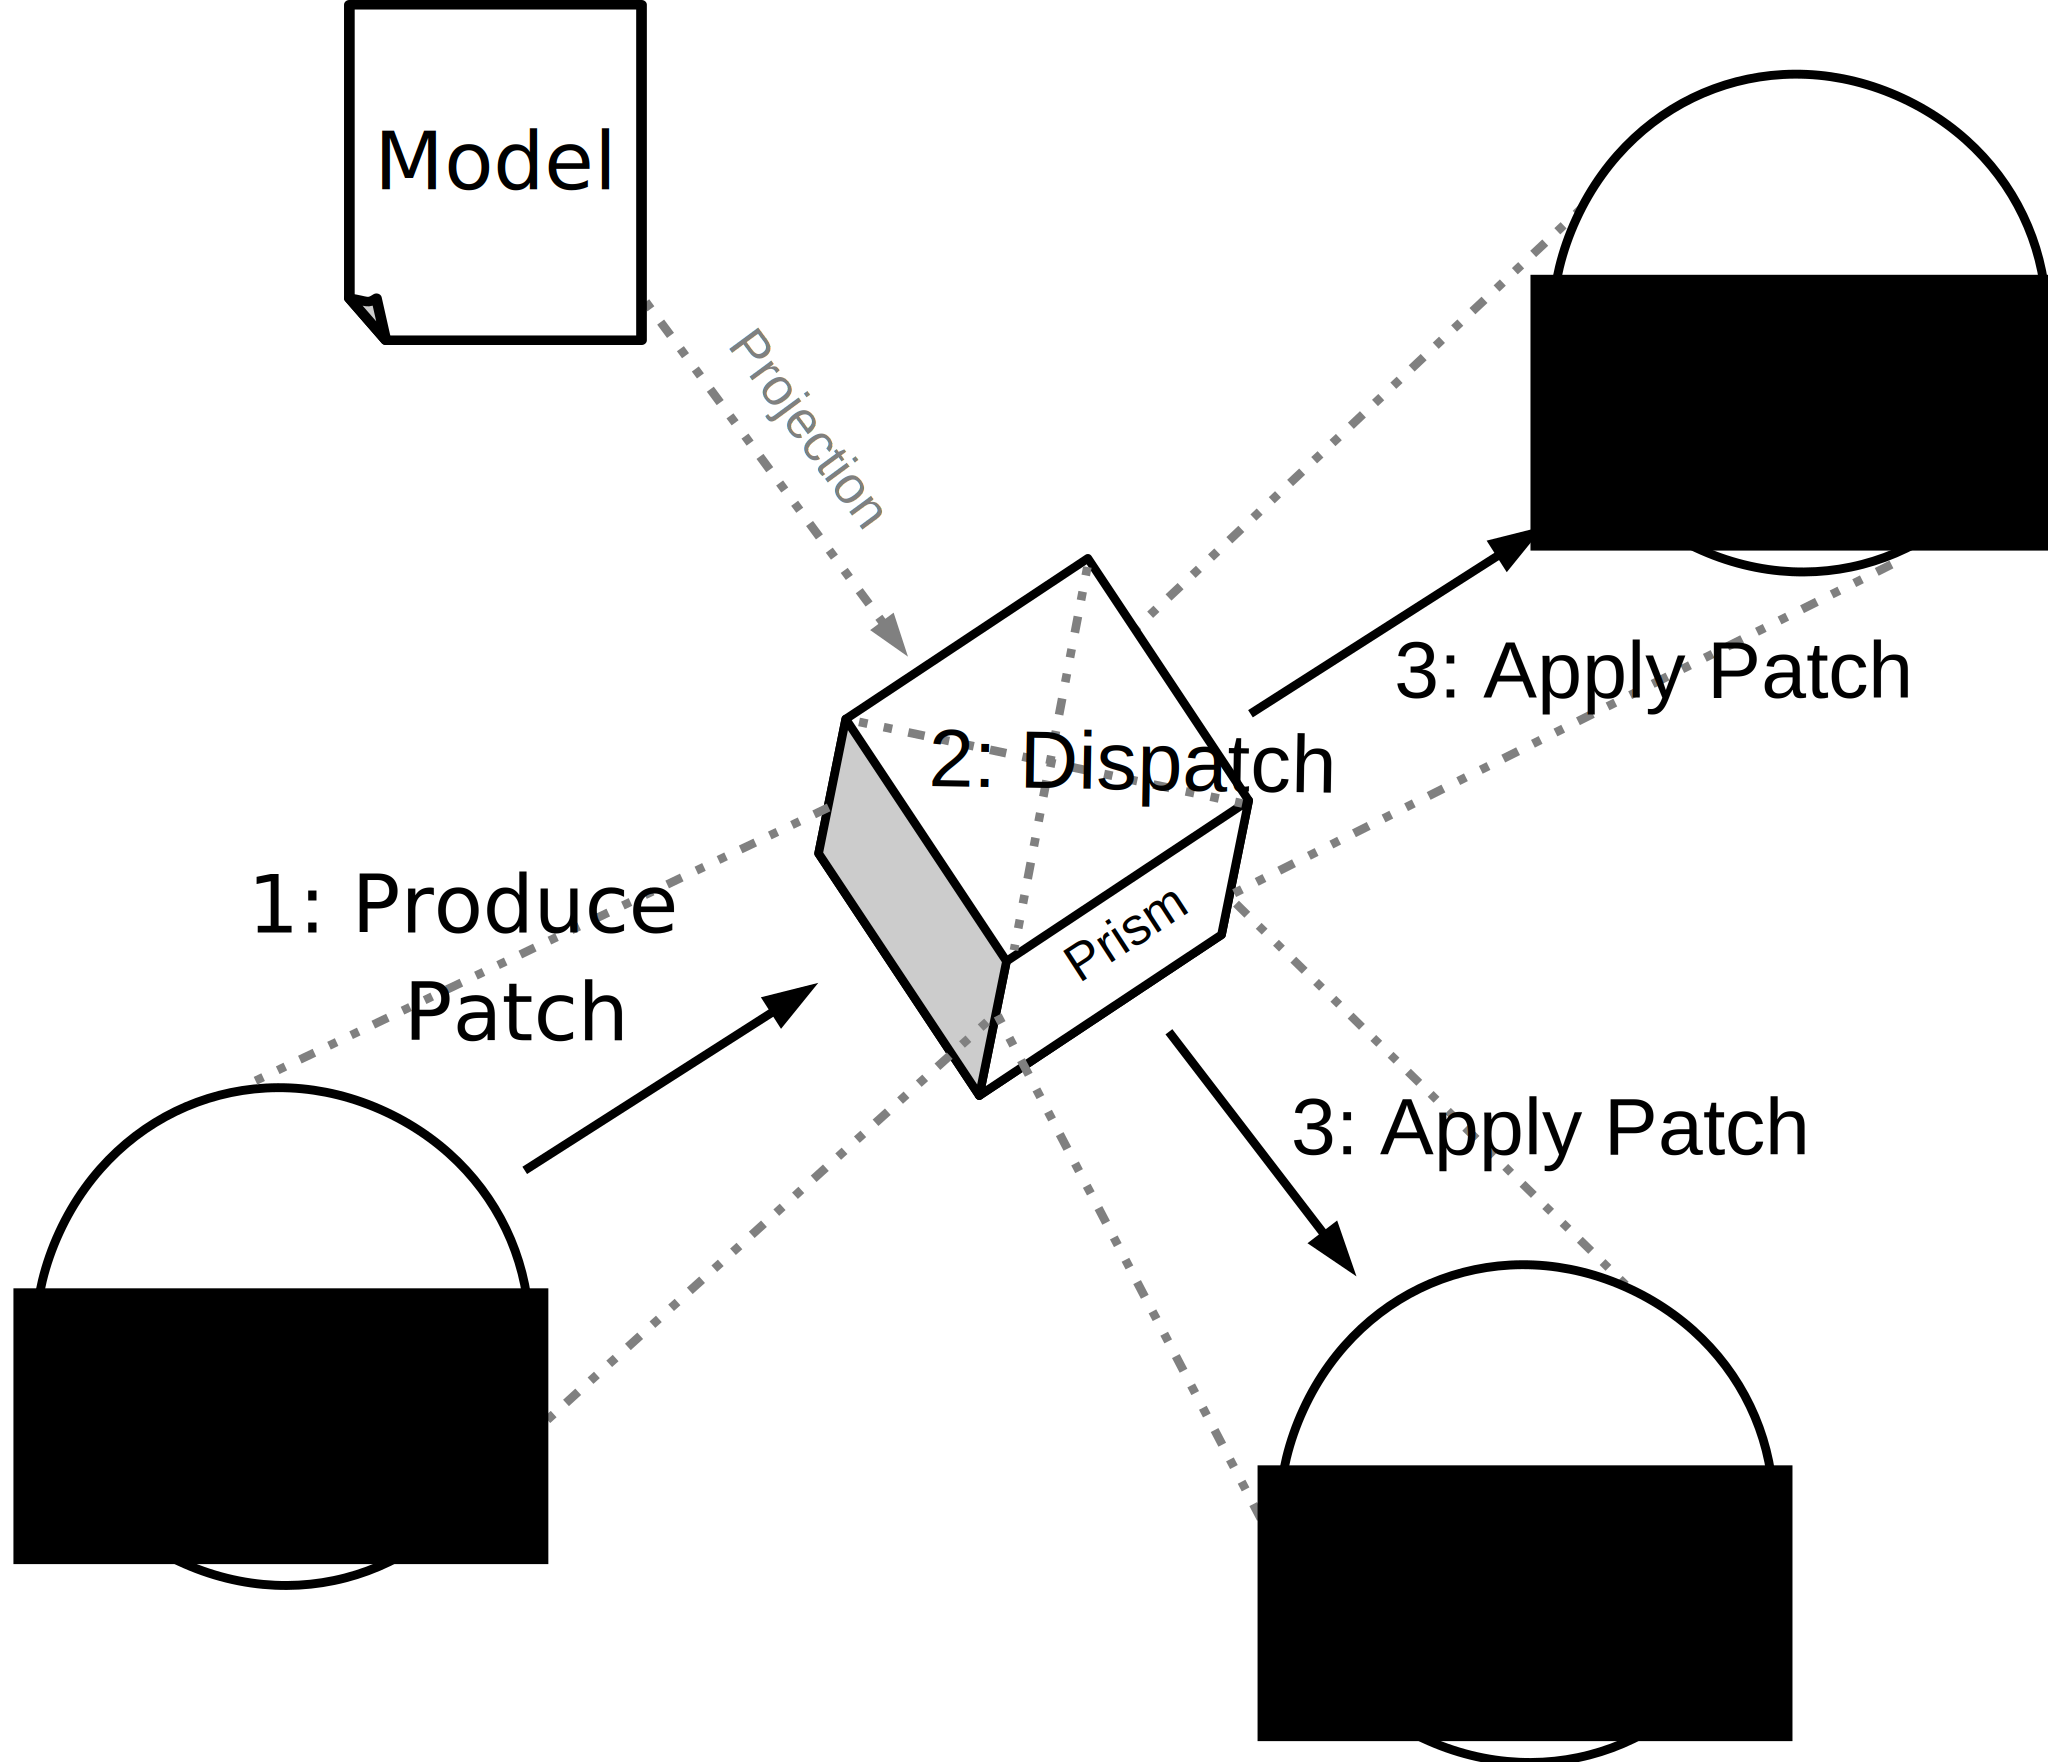
\includegraphics[width=.6\columnwidth]{figures/prism}
	\caption{A model projected in different Technological Spaces}
	\label{fig:prism}
\end{figure}

\begin{figure}
	\centering
	
\includegraphics[width=.8\columnwidth]{figures/concepts}
	\caption{Languages (resp.~models) are projected as shapes (resp.~incarnations) in LVs. Just as models conform to languages, incarnations conform to shapes.\\NB: \emph{projectedAs $\Rightarrow$ realizedBy} or something else?}
	\label{fig:concepts}
\end{figure}

A naive way to bridge different LV would be to define bidirectional transformations between the abstract syntax formalisms of every pair $\langle LV, LV' \rangle$.
Doing so however would break \emph{incrementality}, \ie~it would not be possible to maintain the extra information every TS holds, such as layout in a editor or runtime data when running models.
In our approach, instead, every change occuring on one side is shipped to all the other sides.
The latter then decide which parts of the changes they want to take into account.
An outline, for instance, would probably ignore most of the changes and focus on some of them. Argh.

Bridging multiple TS thus requires to ``align'' in some ways the representation of the AS of a language in these different TS.
As an illustration, the EMF and the Rascal LWB expose fundamental differences:~object-oriented vs. functional, graphs vs. trees, mutable ASG vs. immutable ASTs, cross-references vs. symbolic names, \etc.
However, it is neither possible nor desirable to establish a common formalism upon which various TS would agree:~mapping those is out of reach.

The key underlying idea of our approach is to provide the capability, at any time, to ``project'' a given model in any of its shapes and to synchronize those shapes whenever one of them is updated.
We enable the projection of a given model as an ADT value, to be manipulated in the Rascal TS, or as an Ecore model, to be manipulated in the EMF TS.

Instead, our approach keeps the TS fully independent and builds a communication bus between them.
Both representations of the same model in various TS are kept in memory to allow online synchronization of the same models manipulated by different stakeholders in different shapes.
When a changes occurs on either side, this side is responsible for generating a \emph{patch} (aka. \de or edit script~\cite{rozen2017towards}), that stores the changes on the model that have been realized on this side.
The communication bus then ships this patch to all the other sides.
Every side interprets the patch in its own way to keep the representation synchronized.
On the EMF side, for instance, the patch is interpreted as a set of changes that impact an Ecore model, while on the Rascal side it is interpreted as a set of changes that impact a value conforming to the ADT defining the AS of the language.

It is important to note that each TS may want to preserve certain information across the patches that are specific to the TS.
A textual editor in Rascal, for instance, needs to keep some of the parsing information to maintain layout whenever patches are applied.
So it should be possible to apply the patch while maintaining the extra information specific to a given TS.

Automatically generating language implementations in different TS is beyond the scope of this paper.\footnote{Indeed, this would actually require to build some kind of BX between all AS formalisms; so, nope!} Instead, given various shapes of a language, implemented by hand, we provide the means to automatically synchronize the projections of a model.

\begin{lstlisting}[label=lst:delta-adt, caption={CRUD-like \ds structure definition in Rascal}, language=Rascal]
@doc{A patch consists of a sequence of edits}
alias Patch = tuple[Id root, Edits edits];

@doc{Edits are operations attached to object identities}
alias Edits = lrel[Id obj, Edit edit];

data Edit
  = put(str field, value val)
  | unset(str field)
  | ins(str field, int pos, value val)
  | del(str field, int pos)
  | create(str class) 
  | destroy();
\end{lstlisting}

It is important to note that ``projections'' have no relation whatsoever with projectional editing.
A projection denotes the incarnation of a model in a particular shape of a language.
In \Cref{fig:motivating-fsm}, the lower part depicts three projections of the same \texttt{Button} state machine model in three shapes of the FSM language.
We use the term ``language'' to refer to the specification of a language independently from its realization in a given TS.
A concrete implementation of a language is a ``shape''.
An instance of a shape, \ie~a particular model in a particular TS, is a ``projection'' of a ``virtual'' model.
Metamorphic synchronization refers to the ability to synchronize the projections of a given model for every shapes of a language.

\begin{definition}
A technological space is a collection of tools and an environment defining a coherent space where users can design and use Languages.
\td{There's already a definition of TS that we should reuse (\cf footnote 1 page 1---\citeauthor{kurtev2002technological}~\cite{kurtev2002technological}}
\end{definition}

\begin{definition}
A projection of model is a relation between a conceptual model and its different incarnations in the technological spaces.
All of theses incarnations represent the same model but in different formalisms and technologies.
They are two necessary properties to have a model projection.
\begin{itemize}
	\item incarnations have to be in an equivalent \td{what does ``equivalent'' mean here?} states.
	\item incarnations have to be synchronized, i.e., any change on an incarnation is a change on the conceptual model and thus other incarnations have to apply the same change \td{Isn't that a duplicate of the previous point? Remove the first?}.
\end{itemize}
\end{definition}

\begin{definition}
The equivalence between the state of different incarnations is defined thanks to a Diff operation.
The Diff operation compare two states and output a description of the changes between them.
Two incarnations are in equivalent state if the Diff between a state and an empty state is equal for both incarnation.
Moreover for any change operation applicable to an incarnation, the two incarnations have to be in an equivalent state after the change.
\end{definition}

\begin{definition}
An incarnation is in the context of a model projection what is representing the model in a given technological space.
\end{definition}

\begin{definition}
A prism is the context of a model projection is the mechanism that allows the different incarnations of the model to be in equivalent state and to synchronize.
\end{definition}

\begin{definition}
A shape is a projection of a language in a particular technological space.
\td{Is it equivalent to the language \emph{implementation}?}
An incarnation of a model is conform to a shape of language if both are in the same technological space and if the model is conform to the language.
\end{definition}
    % How
\section{A Shape-Diverse FSM Language}
\label{sec:eval}

To illustrate \prism, we build a shape-diverse FSM language conjointly in Rascal, EMF, and Java.
\Cref{fig:3fsms} depicts the implementation of the abstract syntax of this FSM language in the three LVs.\footnote{The implementation of \prism and the FSM example are available on a companion webpage:~\url{https://github.com/fcoulon/prism/}}
The corresponding incarnations are those given in \Cref{fig:motivating-fsm}.

\begin{figure}[bt]
	\centering
	\begin{subfigure}[b]{.3\columnwidth}
		\begin{lstlisting}[label=lst:fsm-adt, language=Rascal, numbers=none, xleftmargin=0pt, tabsize=1]
data Machine(Id uid) =
	Machine(str name,
		list[State] states,
		Ref[State] initial);

data State(Id uid) =
	State(str name,
		list[Trans] trans);

data Trans(Id uid) =
	Trans(str event,
		Ref[State] target);
		\end{lstlisting}
		\caption{Rascal ADT}
	\end{subfigure}
	\vrule
	\enskip
	\begin{subfigure}[b]{.26\columnwidth}
		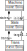
\includegraphics[width=\textwidth]{figures/fsm-mm}
		\caption{Ecore MM}
	\end{subfigure}
	\enskip
	\vrule
	\enskip
	\begin{subfigure}[b]{.35\columnwidth}
		\begin{lstlisting}[label=lst:fsm-api, language=Java, numbers=none, xleftmargin=0pt, tabsize=1]
class Fsm {
	Fsm(String name);
	State init(String name);
	State state(String name);
	Fsm end();
}
class State {
	State state(String name);
	Trans tgt(String name);
	Fsm end();
}
class Trans {
	Trans tgt(String name);
	State on(String event);
	Fsm end();
}
		\end{lstlisting}
		\caption{Java API}
	\end{subfigure}
	\caption{Three shapes of an FSM language; the corresponding incarnations are those depicted in \Cref{fig:motivating-fsm}.}
	\label{fig:3fsms}
\end{figure}

We use Rascal to define a textual editor and a simple transformation that inserts a new state in a machine.
We use EMF to define two graphical editors:~a classical tree editor and a domain-specific representation with Sirius.\footnote{\url{https://www.eclipse.org/sirius/}}
We build the Java API following a simple systematic convention, so as to easily pinpoint which parts of the Java AST have changed (to compute a patch) or need to be updated (to apply a patch).

\prism is used to bridge these different shapes.
Whenever an incarnation of the FSM model is updated, the LV in which the change happens produces a patch (\cf\Cref{lst:delta-adt}) that is shipped to the other LVs through the dispatch mechanism of \prism.
Every LV interprets the patch in its own way to keep its incarnation updated, accounting for the extra information it has to manage (\eg~layouts within the textual and graphical editors).
%A simple matrix, internal to \prism, keeps track of which model each incarnation is projecting to route the patch to the right incarnation.

%Rascal is providing a textual editor, Ecore provides a graphical editor and we used the Java editor for the fluent API.
%In our manipulation we were able to edit an incarnation of a model in one editor and see the change applied in others editors.
%By using an editor, we were able to benefit of the result of the tooling in others incarnations, i.e., using the content assist of Java is also updating other editors.
%We also observe some de-synchronization happening due to the partially unaligned FSM implementation in Java.

While the Rascal and EMF shapes synchronize seamlessly, we noticed a number of challenges with the Java API.
As the Java API inherits the (domain-agnostic) tooling of Java itself, it lacks the domain knowledge necessary to always generate correct patches.
Due to the lack of domain-specific static semantics, a well-formed Java program may indeed produce an ill-formed FSM that cannot be interpreted by the other shapes.
Besides, our prototype implementation does not account for complex string manipulation when invoking the API or use of variables.
However, we believe that these are purely engineering concerns and that enough effort spent on the Java API shape would provide a flawless experience.

%The Java fluent API shape tends to break more easily the synchronization of their incarnations of models than the other shapes.
%Indeed this shape of FSM language is an embedded language and has to rely on the host language for both the tooling and the expressiveness.
%In the case of Java as host language, the validation service provided by the editor has no knowledge about the FSM language.
%It makes harder for the user to detect mistakes such as typo. The FSM model can be in unnoticed dirty state and this can lead to the production of dirty Patches.
%In the opposite the incarnation of the model can receive inapplicable Patches in this technological space.

%Another example in the Java TS of problem encountered is the constraints from the host language.
%We choose to represent a State by the method state() or by the method initial().
%As the initial State is unique, we enforce its declaration as the first method invocation in the FSM.
%This solution solve the uniqueness but enforce the first state to be initial.
%Thus with this representation of FSM, receiving a Patch telling to reference the second state of an FSM as the initial state is not possible due to the expressiveness of the API and this result in the desynchronization of the incarnation of the model.
%
%The inconsistency of the incarnations of a model happen when one of them produce a dirty Patch or when one of them can't apply a Patch.
        % Example
\section{Discussion \& Next Steps}
\label{sec:discussion}
\td{If we write a vision paper, there must be a vision. Next steps? Roadmap? Challenges? What should the reader gain from reading this paper?}
\td{\eg It works here for 3 ``representative'' TS. What should you have in mind if you want to do that for others? What if you want to scale for collaborative/live modeling? \etc}
\begin{itemize}
	\item Our approach goes beyond what is described here. \eg synchronizing an outline view, a debugger, live modeling, w/e; also, we are AS-centric, but one could imagine something radically different;
	\item We don’t care how the list of changes is obtained. Diff is \emph{a} way to get there (as in the Rascal implementation), but obtaining the list of changes through other means (e.g., a transaction on a tree editor in EMF) is just as valid;
	\item Our dispatch is braindead. A better dispatch may enable collaborative editing, distributed synchronization, \etc;
	\item It may or may not be possible to automatically generate a shape from another. \eg~we did it for Ecore $\leftrightarrow$ Rascal;
	\item Transforming context-heavy Java ASTs is challenging; our tool is stupid in that respect; DIY;
	\item We do not really know if our patch formalism is sufficient; what if you want to plug another formalism; is there anything missing?
	\item \cite{lammel2005mappings}
	\item Delta/edit scripts are known (ref?), ``pivot'' formalisms are---infamously---known, we combine both in a new context; why? what do we get from that?
	\item We view this initial contribution as a first step towards \emph{metamorphic DSLs}~\cite{acher2014metamorphic}.
	\item We need a mechanism to valid produced Patches and their interpretations to detect desynchronization of incarnations (what should we do then? roll back? fix Patch? )
    \item The rigidity of SLE must be thought. Must find ways to let the users move agilely from shapes to shapes, and let the designers combine the strengths of multiple LV.
\end{itemize}
  % Opening

\begin{acks}
This work is partially supported by the associate team ALE (\url{http://gemoc.org/ale/}), and the EU's Horizon 2020 Project No. 732223 CROSSMINER.
\end{acks}

\clearpage
\balance
\bibliographystyle{ACM-Reference-Format}
\bibliography{main}

%\clearpage
%\section*{Notes}
%
%\begin{itemize}
%	\item In \Cref{fig:concepts}, projectedAs $\Rightarrow$ realizedBy / materializedBy / something else?
%\end{itemize}

\end{document}
